\documentclass[twoside]{book}

% Packages required by doxygen
\usepackage{fixltx2e}
\usepackage{calc}
\usepackage{doxygen}
\usepackage[export]{adjustbox} % also loads graphicx
\usepackage{graphicx}
\usepackage[utf8]{inputenc}
\usepackage{makeidx}
\usepackage{multicol}
\usepackage{multirow}
\PassOptionsToPackage{warn}{textcomp}
\usepackage{textcomp}
\usepackage[nointegrals]{wasysym}
\usepackage[table]{xcolor}

% Font selection
\usepackage[T1]{fontenc}
\usepackage[scaled=.90]{helvet}
\usepackage{courier}
\usepackage{amssymb}
\usepackage{sectsty}
\renewcommand{\familydefault}{\sfdefault}
\allsectionsfont{%
  \fontseries{bc}\selectfont%
  \color{darkgray}%
}
\renewcommand{\DoxyLabelFont}{%
  \fontseries{bc}\selectfont%
  \color{darkgray}%
}
\newcommand{\+}{\discretionary{\mbox{\scriptsize$\hookleftarrow$}}{}{}}

% Page & text layout
\usepackage{geometry}
\geometry{%
  a4paper,%
  top=2.5cm,%
  bottom=2.5cm,%
  left=2.5cm,%
  right=2.5cm%
}
\tolerance=750
\hfuzz=15pt
\hbadness=750
\setlength{\emergencystretch}{15pt}
\setlength{\parindent}{0cm}
\setlength{\parskip}{0.2cm}
\makeatletter
\renewcommand{\paragraph}{%
  \@startsection{paragraph}{4}{0ex}{-1.0ex}{1.0ex}{%
    \normalfont\normalsize\bfseries\SS@parafont%
  }%
}
\renewcommand{\subparagraph}{%
  \@startsection{subparagraph}{5}{0ex}{-1.0ex}{1.0ex}{%
    \normalfont\normalsize\bfseries\SS@subparafont%
  }%
}
\makeatother

% Headers & footers
\usepackage{fancyhdr}
\pagestyle{fancyplain}
\fancyhead[LE]{\fancyplain{}{\bfseries\thepage}}
\fancyhead[CE]{\fancyplain{}{}}
\fancyhead[RE]{\fancyplain{}{\bfseries\leftmark}}
\fancyhead[LO]{\fancyplain{}{\bfseries\rightmark}}
\fancyhead[CO]{\fancyplain{}{}}
\fancyhead[RO]{\fancyplain{}{\bfseries\thepage}}
\fancyfoot[LE]{\fancyplain{}{}}
\fancyfoot[CE]{\fancyplain{}{}}
\fancyfoot[RE]{\fancyplain{}{\bfseries\scriptsize Generated on Mon Jan 12 2015 10\+:40\+:14 for Giraffe tour by Doxygen }}
\fancyfoot[LO]{\fancyplain{}{\bfseries\scriptsize Generated on Mon Jan 12 2015 10\+:40\+:14 for Giraffe tour by Doxygen }}
\fancyfoot[CO]{\fancyplain{}{}}
\fancyfoot[RO]{\fancyplain{}{}}
\renewcommand{\footrulewidth}{0.4pt}
\renewcommand{\chaptermark}[1]{%
  \markboth{#1}{}%
}
\renewcommand{\sectionmark}[1]{%
  \markright{\thesection\ #1}%
}

% Indices & bibliography
\usepackage{natbib}
\usepackage[titles]{tocloft}
\setcounter{tocdepth}{3}
\setcounter{secnumdepth}{5}
\makeindex

% Hyperlinks (required, but should be loaded last)
\usepackage{ifpdf}
\ifpdf
  \usepackage[pdftex,pagebackref=true]{hyperref}
\else
  \usepackage[ps2pdf,pagebackref=true]{hyperref}
\fi
\hypersetup{%
  colorlinks=true,%
  linkcolor=blue,%
  citecolor=blue,%
  unicode%
}

% Custom commands
\newcommand{\clearemptydoublepage}{%
  \newpage{\pagestyle{empty}\cleardoublepage}%
}


%===== C O N T E N T S =====

\begin{document}

% Titlepage & ToC
\hypersetup{pageanchor=false,
             bookmarks=true,
             bookmarksnumbered=true,
             pdfencoding=unicode
            }
\pagenumbering{roman}
\begin{titlepage}
\vspace*{7cm}
\begin{center}%
{\Large Giraffe tour }\\
\vspace*{1cm}
{\large Generated by Doxygen 1.8.9.1}\\
\vspace*{0.5cm}
{\small Mon Jan 12 2015 10:40:14}\\
\end{center}
\end{titlepage}
\clearemptydoublepage
\tableofcontents
\clearemptydoublepage
\pagenumbering{arabic}
\hypersetup{pageanchor=true}

%--- Begin generated contents ---
\chapter{Hierarchical Index}
\section{Class Hierarchy}
This inheritance list is sorted roughly, but not completely, alphabetically\+:\begin{DoxyCompactList}
\item \contentsline{section}{Excursion}{\pageref{class_excursion}}{}
\begin{DoxyCompactList}
\item \contentsline{section}{Multiday\+Excursion}{\pageref{class_multiday_excursion}}{}
\item \contentsline{section}{Oneday\+Excursion}{\pageref{class_oneday_excursion}}{}
\end{DoxyCompactList}
\item \contentsline{section}{Item}{\pageref{class_item}}{}
\item \contentsline{section}{mvector$<$ T $>$}{\pageref{classmvector}}{}
\item \contentsline{section}{myiterator$<$ My\+Type $>$}{\pageref{classmyiterator}}{}
\item \contentsline{section}{myiterator\+\_\+const$<$ T $>$}{\pageref{classmyiterator__const}}{}
\item \contentsline{section}{myvector$<$ T $>$}{\pageref{classmyvector}}{}
\item \contentsline{section}{myvectorit$<$ T $>$}{\pageref{classmyvectorit}}{}
\item \contentsline{section}{Record}{\pageref{struct_record}}{}
\item \contentsline{section}{Route}{\pageref{class_route}}{}
\item \contentsline{section}{Table\+Iterator}{\pageref{class_table_iterator}}{}
\item \contentsline{section}{Vector\+Table}{\pageref{class_vector_table}}{}
\end{DoxyCompactList}

\chapter{Class Index}
\section{Class List}
Here are the classes, structs, unions and interfaces with brief descriptions\+:\begin{DoxyCompactList}
\item\contentsline{section}{\hyperlink{class_excursion}{Excursion} }{\pageref{class_excursion}}{}
\item\contentsline{section}{\hyperlink{class_item}{Item} }{\pageref{class_item}}{}
\item\contentsline{section}{\hyperlink{class_multiday_excursion}{Multiday\+Excursion} }{\pageref{class_multiday_excursion}}{}
\item\contentsline{section}{\hyperlink{classmvector}{mvector$<$ T $>$} }{\pageref{classmvector}}{}
\item\contentsline{section}{\hyperlink{classmyiterator}{myiterator$<$ My\+Type $>$} \\*класс итератор }{\pageref{classmyiterator}}{}
\item\contentsline{section}{\hyperlink{classmyiterator__const}{myiterator\+\_\+const$<$ T $>$} \\*Класс конст.\+итератор }{\pageref{classmyiterator__const}}{}
\item\contentsline{section}{\hyperlink{classmyvector}{myvector$<$ T $>$} \\*Класс вектор }{\pageref{classmyvector}}{}
\item\contentsline{section}{\hyperlink{classmyvectorit}{myvectorit$<$ T $>$} }{\pageref{classmyvectorit}}{}
\item\contentsline{section}{\hyperlink{class_oneday_excursion}{Oneday\+Excursion} }{\pageref{class_oneday_excursion}}{}
\item\contentsline{section}{\hyperlink{struct_record}{Record} }{\pageref{struct_record}}{}
\item\contentsline{section}{\hyperlink{class_route}{Route} }{\pageref{class_route}}{}
\item\contentsline{section}{\hyperlink{class_table_iterator}{Table\+Iterator} }{\pageref{class_table_iterator}}{}
\item\contentsline{section}{\hyperlink{class_vector_table}{Vector\+Table} }{\pageref{class_vector_table}}{}
\end{DoxyCompactList}

\chapter{Class Documentation}
\hypertarget{class_excursion}{}\section{Excursion Class Reference}
\label{class_excursion}\index{Excursion@{Excursion}}
Inheritance diagram for Excursion\+:\begin{figure}[H]
\begin{center}
\leavevmode
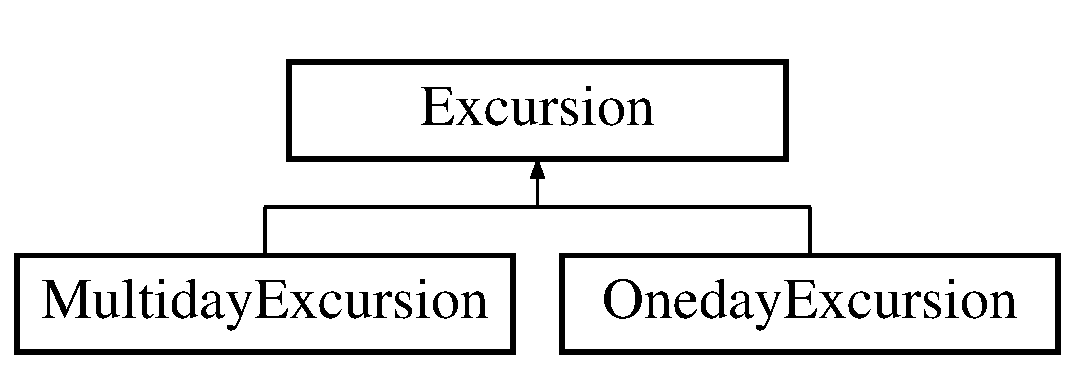
\includegraphics[height=2.000000cm]{class_excursion}
\end{center}
\end{figure}
\subsection*{Public Member Functions}
\begin{DoxyCompactItemize}
\item 
\hypertarget{class_excursion_a2a3a954d1938a78121ae94c85edc5252}{}{\bfseries Excursion} (const string \&name, const float \&cost, const unsigned int \&year, const unsigned int \&month, const unsigned int \&day, const unsigned int \&hour, const unsigned int \&min, const unsigned int \&max\+Tourists, const unsigned int \&sold\+Seats)\label{class_excursion_a2a3a954d1938a78121ae94c85edc5252}

\item 
\hypertarget{class_excursion_ad4eea52ed5b6a747139aedf0dce40e90}{}virtual \hyperlink{class_excursion}{Excursion} $\ast$ {\bfseries clone} () const =0\label{class_excursion_ad4eea52ed5b6a747139aedf0dce40e90}

\item 
\hypertarget{class_excursion_af9730feecd3c87c84db1ca87b91a9b5a}{}virtual void {\bfseries set\+Name} (const string \&name)\label{class_excursion_af9730feecd3c87c84db1ca87b91a9b5a}

\item 
\hypertarget{class_excursion_a14001909d85d73f4d28009343d387da2}{}virtual void {\bfseries set\+Name} (std\+::istream \&is)\label{class_excursion_a14001909d85d73f4d28009343d387da2}

\item 
\hypertarget{class_excursion_aa7593c43269c8a201f2d9600c9f6a883}{}virtual string {\bfseries get\+Name} () const \label{class_excursion_aa7593c43269c8a201f2d9600c9f6a883}

\item 
\hypertarget{class_excursion_acdab32c88cd3f338508fa8f301de5c43}{}virtual void {\bfseries set\+Date\+Start} (const unsigned int \&year, const unsigned int \&month, const unsigned int \&day, const unsigned int \&hour, const unsigned int \&min)\label{class_excursion_acdab32c88cd3f338508fa8f301de5c43}

\item 
\hypertarget{class_excursion_a2145b43efb2dadd105d15e59fa462190}{}virtual tm {\bfseries get\+Date\+Start} () const \label{class_excursion_a2145b43efb2dadd105d15e59fa462190}

\item 
\hypertarget{class_excursion_a844bd4f17be0f232464c8da55106304c}{}virtual void {\bfseries set\+Cost} (const float \&cost)\label{class_excursion_a844bd4f17be0f232464c8da55106304c}

\item 
\hypertarget{class_excursion_ae6d87d9e36db67922f56c6a89ef1ee92}{}virtual float {\bfseries get\+Cost} () const \label{class_excursion_ae6d87d9e36db67922f56c6a89ef1ee92}

\item 
\hypertarget{class_excursion_a9bb8a4ab1315a761e5e77916583395a0}{}virtual void {\bfseries set\+Max\+Tourists} (const unsigned int \&max\+Tourists)\label{class_excursion_a9bb8a4ab1315a761e5e77916583395a0}

\item 
\hypertarget{class_excursion_ad26a68806010d73090ff692d589cd6db}{}virtual void {\bfseries set\+Sold\+Seats} (const unsigned int \&sold\+Seats)\label{class_excursion_ad26a68806010d73090ff692d589cd6db}

\item 
\hypertarget{class_excursion_a637bb734067850afdb8e03387053ed1b}{}virtual void {\bfseries sell\+Seats} (const unsigned int \&sell\+Seats)\label{class_excursion_a637bb734067850afdb8e03387053ed1b}

\item 
\hypertarget{class_excursion_a745a8ad5fc4f49c138ea1f02ffd8a2bf}{}virtual void {\bfseries free\+Seats} (const unsigned int \&free\+Seats)\label{class_excursion_a745a8ad5fc4f49c138ea1f02ffd8a2bf}

\item 
\hypertarget{class_excursion_a7c7b692a96bccdaed968560c0d64ff39}{}virtual unsigned int {\bfseries get\+Sold\+Seats} () const \label{class_excursion_a7c7b692a96bccdaed968560c0d64ff39}

\item 
\hypertarget{class_excursion_a47c133a0994313c97ff30629de2c9967}{}virtual unsigned int {\bfseries get\+Max\+Tourists} () const \label{class_excursion_a47c133a0994313c97ff30629de2c9967}

\item 
\hypertarget{class_excursion_adf535a29b8de27c166ac4cf9ce6dbbe5}{}std\+::string {\bfseries e\+Get\+Name\+Place} ()\label{class_excursion_adf535a29b8de27c166ac4cf9ce6dbbe5}

\end{DoxyCompactItemize}
\subsection*{Protected Member Functions}
\begin{DoxyCompactItemize}
\item 
\hypertarget{class_excursion_a3e80eaf524f6380dffa15c309a4fe9b1}{}virtual std\+::ostream \& {\bfseries show} (std\+::ostream \&os) const =0\label{class_excursion_a3e80eaf524f6380dffa15c309a4fe9b1}

\item 
\hypertarget{class_excursion_a99997fabe3a8997ec0f9fe9c32475c9b}{}virtual std\+::istream \& {\bfseries get} (std\+::istream \&is)=0\label{class_excursion_a99997fabe3a8997ec0f9fe9c32475c9b}

\end{DoxyCompactItemize}
\subsection*{Friends}
\begin{DoxyCompactItemize}
\item 
\hypertarget{class_excursion_af70b8892ec207843abcaf672f510a890}{}std\+::ostream \& {\bfseries operator$<$$<$} (std\+::ostream \&os, const \hyperlink{class_excursion}{Excursion} \&excursion)\label{class_excursion_af70b8892ec207843abcaf672f510a890}

\item 
\hypertarget{class_excursion_afdf9047952f2241c224581955c23bda1}{}std\+::istream \& {\bfseries operator$>$$>$} (std\+::istream \&is, \hyperlink{class_excursion}{Excursion} \&excursion)\label{class_excursion_afdf9047952f2241c224581955c23bda1}

\end{DoxyCompactItemize}


The documentation for this class was generated from the following files\+:\begin{DoxyCompactItemize}
\item 
Excursion.\+h\item 
Excursion.\+cpp\end{DoxyCompactItemize}

\hypertarget{class_item}{}\section{Item Class Reference}
\label{class_item}\index{Item@{Item}}
\subsection*{Public Member Functions}
\begin{DoxyCompactItemize}
\item 
\hyperlink{class_item_a92fbc538cf5a7e47e1129f33a6c53453}{Item} (const string \&name\+Place, const string \&name\+Item, const unsigned int \&hour, const unsigned int \&min, const unsigned int \&duration)
\begin{DoxyCompactList}\small\item\em конструктор пункта по умолчанию (название населенного пункта -\/ None, название экскурсионного объекта -\/ None, дата и время -\/ текущее время \end{DoxyCompactList}\item 
\hypertarget{class_item_a8bdb9e933891e13672b1979dbc51401d}{}void \hyperlink{class_item_a8bdb9e933891e13672b1979dbc51401d}{set\+Name\+Place} (const string \&name\+Place)\label{class_item_a8bdb9e933891e13672b1979dbc51401d}

\begin{DoxyCompactList}\small\item\em диструктор пункта \end{DoxyCompactList}\item 
\hypertarget{class_item_adb511922ae79a79c40f3542ae457fac4}{}void \hyperlink{class_item_adb511922ae79a79c40f3542ae457fac4}{set\+Name\+Place} (std\+::istream \&is)\label{class_item_adb511922ae79a79c40f3542ae457fac4}

\begin{DoxyCompactList}\small\item\em ввод названия населенного пункта \end{DoxyCompactList}\item 
\hypertarget{class_item_a18f8c9c7e6fc0a2326d75b7c1857bc51}{}string \hyperlink{class_item_a18f8c9c7e6fc0a2326d75b7c1857bc51}{get\+Name\+Place} () const \label{class_item_a18f8c9c7e6fc0a2326d75b7c1857bc51}

\begin{DoxyCompactList}\small\item\em ввод названия населенного пункта в поток \end{DoxyCompactList}\item 
\hypertarget{class_item_af7bca1854d89b1d7315cf9b37ec41aec}{}void \hyperlink{class_item_af7bca1854d89b1d7315cf9b37ec41aec}{set\+Name\+Item} (const string \&name\+Item)\label{class_item_af7bca1854d89b1d7315cf9b37ec41aec}

\begin{DoxyCompactList}\small\item\em вывод название населенного пунска \end{DoxyCompactList}\item 
\hypertarget{class_item_a80e0444dcf74fa46cc93acf03ac785f9}{}void \hyperlink{class_item_a80e0444dcf74fa46cc93acf03ac785f9}{set\+Name\+Item} (std\+::istream \&is)\label{class_item_a80e0444dcf74fa46cc93acf03ac785f9}

\begin{DoxyCompactList}\small\item\em ввод названия экскурсионного объекта \end{DoxyCompactList}\item 
\hypertarget{class_item_ac1d5462440e6e7ce3eb4c233a01572bb}{}string \hyperlink{class_item_ac1d5462440e6e7ce3eb4c233a01572bb}{get\+Name\+Item} () const \label{class_item_ac1d5462440e6e7ce3eb4c233a01572bb}

\begin{DoxyCompactList}\small\item\em ввод названия экскурсиооного объекта в поток \end{DoxyCompactList}\item 
\hypertarget{class_item_ae132cf1854d8fe37d4e04251b70a1947}{}void \hyperlink{class_item_ae132cf1854d8fe37d4e04251b70a1947}{set\+Time\+Start} (const unsigned int \&hour, const unsigned int \&min)\label{class_item_ae132cf1854d8fe37d4e04251b70a1947}

\begin{DoxyCompactList}\small\item\em вывод названия экскурсиооного объекта \end{DoxyCompactList}\item 
\hypertarget{class_item_a5ab6e4d465de10ebe2cac323f392f111}{}void \hyperlink{class_item_a5ab6e4d465de10ebe2cac323f392f111}{set\+Time\+Start} (std\+::istream \&is)\label{class_item_a5ab6e4d465de10ebe2cac323f392f111}

\begin{DoxyCompactList}\small\item\em ввод времени начала экскурсии \end{DoxyCompactList}\item 
\hypertarget{class_item_a4947c0cc15e90d0271927c94f91e2367}{}tm \hyperlink{class_item_a4947c0cc15e90d0271927c94f91e2367}{get\+Time\+Start} () const \label{class_item_a4947c0cc15e90d0271927c94f91e2367}

\begin{DoxyCompactList}\small\item\em ввод времени начала экскурсии в поток \end{DoxyCompactList}\item 
\hypertarget{class_item_a5d8a338a95052112bfd9e88b602f263b}{}void \hyperlink{class_item_a5d8a338a95052112bfd9e88b602f263b}{set\+Duration} (const unsigned int \&duration)\label{class_item_a5d8a338a95052112bfd9e88b602f263b}

\begin{DoxyCompactList}\small\item\em вывод времени начала экскурсии \end{DoxyCompactList}\item 
\hypertarget{class_item_aebe178d9136a81916fd7f56be7245293}{}void \hyperlink{class_item_aebe178d9136a81916fd7f56be7245293}{set\+Duration} (std\+::istream \&is)\label{class_item_aebe178d9136a81916fd7f56be7245293}

\begin{DoxyCompactList}\small\item\em ввод продолжительности экскурсии \end{DoxyCompactList}\item 
\hypertarget{class_item_aaed2c5908376d037db6df319bc2ec2c5}{}int \hyperlink{class_item_aaed2c5908376d037db6df319bc2ec2c5}{get\+Duration} () const \label{class_item_aaed2c5908376d037db6df319bc2ec2c5}

\begin{DoxyCompactList}\small\item\em ввод продолжительности экскурсии в поток \end{DoxyCompactList}\end{DoxyCompactItemize}
\subsection*{Friends}
\begin{DoxyCompactItemize}
\item 
\hypertarget{class_item_a2f8f92eea1c84a32bafc197830873f63}{}std\+::ostream \& \hyperlink{class_item_a2f8f92eea1c84a32bafc197830873f63}{operator$<$$<$} (std\+::ostream \&os, const \hyperlink{class_item}{Item} \&item)\label{class_item_a2f8f92eea1c84a32bafc197830873f63}

\begin{DoxyCompactList}\small\item\em вывод продолжительности экскурсии \end{DoxyCompactList}\item 
\hypertarget{class_item_abe2a847b86fc0c1f591d69fc7612bb5f}{}std\+::istream \& \hyperlink{class_item_abe2a847b86fc0c1f591d69fc7612bb5f}{operator$>$$>$} (std\+::istream \&is, \hyperlink{class_item}{Item} \&item)\label{class_item_abe2a847b86fc0c1f591d69fc7612bb5f}

\begin{DoxyCompactList}\small\item\em перегруженный оператор вывда \end{DoxyCompactList}\end{DoxyCompactItemize}


\subsection{Constructor \& Destructor Documentation}
\hypertarget{class_item_a92fbc538cf5a7e47e1129f33a6c53453}{}\index{Item@{Item}!Item@{Item}}
\index{Item@{Item}!Item@{Item}}
\subsubsection[{Item}]{\setlength{\rightskip}{0pt plus 5cm}Item\+::\+Item (
\begin{DoxyParamCaption}
\item[{const string \&}]{name\+Place, }
\item[{const string \&}]{name\+Item, }
\item[{const unsigned int \&}]{hour, }
\item[{const unsigned int \&}]{min, }
\item[{const unsigned int \&}]{duration}
\end{DoxyParamCaption}
)}\label{class_item_a92fbc538cf5a7e47e1129f33a6c53453}


конструктор пункта по умолчанию (название населенного пункта -\/ None, название экскурсионного объекта -\/ None, дата и время -\/ текущее время 


\begin{DoxyParams}{Parameters}
{\em name\+Item} & конструктор пункта \\
\hline
\end{DoxyParams}


The documentation for this class was generated from the following files\+:\begin{DoxyCompactItemize}
\item 
item.\+h\item 
item.\+cpp\end{DoxyCompactItemize}

\hypertarget{class_multiday_excursion}{}\section{Multiday\+Excursion Class Reference}
\label{class_multiday_excursion}\index{Multiday\+Excursion@{Multiday\+Excursion}}
Inheritance diagram for Multiday\+Excursion\+:\begin{figure}[H]
\begin{center}
\leavevmode
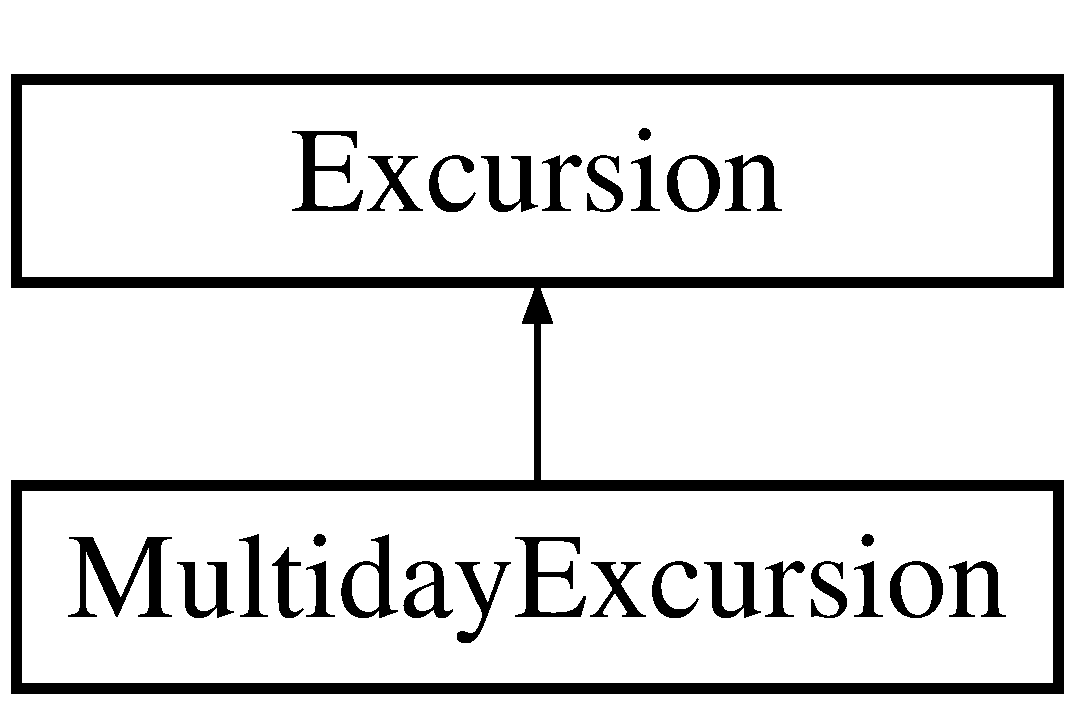
\includegraphics[height=2.000000cm]{class_multiday_excursion}
\end{center}
\end{figure}
\subsection*{Public Member Functions}
\begin{DoxyCompactItemize}
\item 
\hypertarget{class_multiday_excursion_a665b8ff500f3f677f4236c0e9681d0ab}{}\hyperlink{class_multiday_excursion_a665b8ff500f3f677f4236c0e9681d0ab}{Multiday\+Excursion} (const unsigned int \&amount\+Days)\label{class_multiday_excursion_a665b8ff500f3f677f4236c0e9681d0ab}

\begin{DoxyCompactList}\small\item\em конструктор многодневной экскурсии по умолчанию \end{DoxyCompactList}\item 
\hypertarget{class_multiday_excursion_a0f41663ad3b87b0c117d22caa404c4bf}{}\hyperlink{class_multiday_excursion_a0f41663ad3b87b0c117d22caa404c4bf}{Multiday\+Excursion} (const unsigned int \&amount\+Days, \hyperlink{class_route}{Route} $\ast$routes)\label{class_multiday_excursion_a0f41663ad3b87b0c117d22caa404c4bf}

\begin{DoxyCompactList}\small\item\em конструктор многодневной экскурсии по количеству дней \end{DoxyCompactList}\item 
\hypertarget{class_multiday_excursion_ac96c4846502a92d9938c8f93bb368b3c}{}\hyperlink{class_multiday_excursion_ac96c4846502a92d9938c8f93bb368b3c}{Multiday\+Excursion} (const \hyperlink{class_multiday_excursion}{Multiday\+Excursion} \&multiday\+Excursion)\label{class_multiday_excursion_ac96c4846502a92d9938c8f93bb368b3c}

\begin{DoxyCompactList}\small\item\em конструктор многодневной экскурсии по маршрута и количеству дней \end{DoxyCompactList}\item 
\hypertarget{class_multiday_excursion_a445b5758b3b56b57aeb1583e2104abcc}{}\hyperlink{class_multiday_excursion_a445b5758b3b56b57aeb1583e2104abcc}{Multiday\+Excursion} (const unsigned int \&amount\+Days, const string \&name, const float \&cost, const unsigned int \&year, const unsigned int \&month, const unsigned int \&day, const unsigned int \&hour, const unsigned int \&min, const unsigned int \&max\+Tourists, const unsigned int \&sold\+Seats)\label{class_multiday_excursion_a445b5758b3b56b57aeb1583e2104abcc}

\begin{DoxyCompactList}\small\item\em копирующий конструктор \end{DoxyCompactList}\item 
\hypertarget{class_multiday_excursion_a976b2d33561989ae2febedcb9de2c9b6}{}\hyperlink{class_multiday_excursion_a976b2d33561989ae2febedcb9de2c9b6}{Multiday\+Excursion} (const unsigned int \&amount\+Days, const string \&name, const float \&cost, const unsigned int \&year, const unsigned int \&month, const unsigned int \&day, const unsigned int \&hour, const unsigned int \&min, const unsigned int \&max\+Tourists, const unsigned int \&sold\+Seats, \hyperlink{class_route}{Route} $\ast$routes)\label{class_multiday_excursion_a976b2d33561989ae2febedcb9de2c9b6}

\begin{DoxyCompactList}\small\item\em конструктор многодневаной экскурсии \end{DoxyCompactList}\item 
\hypertarget{class_multiday_excursion_acdfb7139fe048a79c722bd2ec7cf6826}{}\hyperlink{class_multiday_excursion_acdfb7139fe048a79c722bd2ec7cf6826}{$\sim$\+Multiday\+Excursion} ()\label{class_multiday_excursion_acdfb7139fe048a79c722bd2ec7cf6826}

\begin{DoxyCompactList}\small\item\em конструктор многодневной экскурсии \end{DoxyCompactList}\item 
\hypertarget{class_multiday_excursion_ae9bbf0deba8c6c92b0c735f329df33dc}{}\hyperlink{class_multiday_excursion}{Multiday\+Excursion} \& \hyperlink{class_multiday_excursion_ae9bbf0deba8c6c92b0c735f329df33dc}{operator=} (const \hyperlink{class_multiday_excursion}{Multiday\+Excursion} \&multiday\+Excursion)\label{class_multiday_excursion_ae9bbf0deba8c6c92b0c735f329df33dc}

\begin{DoxyCompactList}\small\item\em диструктор \end{DoxyCompactList}\item 
\hypertarget{class_multiday_excursion_a21290677ebe9b924ed9e1d6cdb72d2c9}{}virtual \hyperlink{class_multiday_excursion}{Multiday\+Excursion} $\ast$ \hyperlink{class_multiday_excursion_a21290677ebe9b924ed9e1d6cdb72d2c9}{clone} () const \label{class_multiday_excursion_a21290677ebe9b924ed9e1d6cdb72d2c9}

\begin{DoxyCompactList}\small\item\em перегруженный оператор ввода \end{DoxyCompactList}\item 
\hypertarget{class_multiday_excursion_abbe3d509718fd64e666f4e8aabee44be}{}void \hyperlink{class_multiday_excursion_abbe3d509718fd64e666f4e8aabee44be}{set\+Amount\+Days} (const unsigned int \&amount\+Days)\label{class_multiday_excursion_abbe3d509718fd64e666f4e8aabee44be}

\begin{DoxyCompactList}\small\item\em метод клонирующий многодневную экскурсию \end{DoxyCompactList}\item 
\hypertarget{class_multiday_excursion_a03bb448d818bb5fc2609be41dc2b9cfc}{}void \hyperlink{class_multiday_excursion_a03bb448d818bb5fc2609be41dc2b9cfc}{set\+Amount\+Days} (std\+::istream \&is)\label{class_multiday_excursion_a03bb448d818bb5fc2609be41dc2b9cfc}

\begin{DoxyCompactList}\small\item\em ввод количества дней \end{DoxyCompactList}\item 
\hypertarget{class_multiday_excursion_a7c91b6c4154380468ebcc65df69f9c49}{}void \hyperlink{class_multiday_excursion_a7c91b6c4154380468ebcc65df69f9c49}{set\+Routes} (const unsigned int \&anount\+Days, \hyperlink{class_route}{Route} $\ast$routes)\label{class_multiday_excursion_a7c91b6c4154380468ebcc65df69f9c49}

\begin{DoxyCompactList}\small\item\em ввод количества дней в поток \end{DoxyCompactList}\item 
\hypertarget{class_multiday_excursion_a320d3c233d53ae04e08cfa54ca002e7a}{}void \hyperlink{class_multiday_excursion_a320d3c233d53ae04e08cfa54ca002e7a}{set\+Route} (const unsigned int \&n, const \hyperlink{class_route}{Route} \&route)\label{class_multiday_excursion_a320d3c233d53ae04e08cfa54ca002e7a}

\begin{DoxyCompactList}\small\item\em ввод маршрутов \end{DoxyCompactList}\item 
\hypertarget{class_multiday_excursion_a43046d664d21e9783e8cdad17e75ce93}{}\hyperlink{class_route}{Route} \& \hyperlink{class_multiday_excursion_a43046d664d21e9783e8cdad17e75ce93}{get\+Route} (const unsigned int \&n)\label{class_multiday_excursion_a43046d664d21e9783e8cdad17e75ce93}

\begin{DoxyCompactList}\small\item\em ввод одного маршрута \end{DoxyCompactList}\item 
\hypertarget{class_multiday_excursion_afb755ee592591f9b53f94b7febdc6169}{}\hyperlink{class_route}{Route} $\ast$ \hyperlink{class_multiday_excursion_afb755ee592591f9b53f94b7febdc6169}{get\+Routes} ()\label{class_multiday_excursion_afb755ee592591f9b53f94b7febdc6169}

\begin{DoxyCompactList}\small\item\em вывод маршрута \end{DoxyCompactList}\item 
\hypertarget{class_multiday_excursion_a93a69740a32cd61c790da4ab8eb08405}{}unsigned int \hyperlink{class_multiday_excursion_a93a69740a32cd61c790da4ab8eb08405}{get\+Amount\+Days} () const \label{class_multiday_excursion_a93a69740a32cd61c790da4ab8eb08405}

\begin{DoxyCompactList}\small\item\em вывод всех маршрутов \end{DoxyCompactList}\end{DoxyCompactItemize}
\subsection*{Protected Member Functions}
\begin{DoxyCompactItemize}
\item 
\hypertarget{class_multiday_excursion_a14615b65c63d94d098ea9d0632cd7a89}{}virtual std\+::ostream \& \hyperlink{class_multiday_excursion_a14615b65c63d94d098ea9d0632cd7a89}{show} (std\+::ostream \&os) const \label{class_multiday_excursion_a14615b65c63d94d098ea9d0632cd7a89}

\begin{DoxyCompactList}\small\item\em вывод количества дней \end{DoxyCompactList}\item 
\hypertarget{class_multiday_excursion_a6b76291f98f0a5e5cf16cca45fa40000}{}virtual std\+::istream \& \hyperlink{class_multiday_excursion_a6b76291f98f0a5e5cf16cca45fa40000}{get} (std\+::istream \&is)\label{class_multiday_excursion_a6b76291f98f0a5e5cf16cca45fa40000}

\begin{DoxyCompactList}\small\item\em вывод информации о многодневной экскурсии \end{DoxyCompactList}\end{DoxyCompactItemize}
\subsection*{Friends}
\begin{DoxyCompactItemize}
\item 
\hypertarget{class_multiday_excursion_ad4cff9f5a54337cfca11d2e94bf6478e}{}std\+::ostream \& \hyperlink{class_multiday_excursion_ad4cff9f5a54337cfca11d2e94bf6478e}{operator$<$$<$} (std\+::ostream \&os, \hyperlink{class_multiday_excursion}{Multiday\+Excursion} \&multiday\+Excursion)\label{class_multiday_excursion_ad4cff9f5a54337cfca11d2e94bf6478e}

\begin{DoxyCompactList}\small\item\em перегруженный оператор присваивания \end{DoxyCompactList}\item 
\hypertarget{class_multiday_excursion_a154defda96fd2b2c3dad2abf8cfd6fb8}{}std\+::istream \& \hyperlink{class_multiday_excursion_a154defda96fd2b2c3dad2abf8cfd6fb8}{operator$>$$>$} (std\+::istream \&is, \hyperlink{class_multiday_excursion}{Multiday\+Excursion} \&multiday\+Excursion)\label{class_multiday_excursion_a154defda96fd2b2c3dad2abf8cfd6fb8}

\begin{DoxyCompactList}\small\item\em перегруженный оператор вывода \end{DoxyCompactList}\end{DoxyCompactItemize}


The documentation for this class was generated from the following files\+:\begin{DoxyCompactItemize}
\item 
multiday\+\_\+excursion.\+h\item 
multiday\+\_\+excursion.\+cpp\end{DoxyCompactItemize}

\hypertarget{classmvector}{}\section{mvector$<$ T $>$ Class Template Reference}
\label{classmvector}\index{mvector$<$ T $>$@{mvector$<$ T $>$}}
\subsection*{Public Types}
\begin{DoxyCompactItemize}
\item 
\hypertarget{classmvector_a70ffcfd6b41c02cf9fe1921521b01bdc}{}typedef \hyperlink{classmyvectorit}{myvectorit}$<$ T $>$ {\bfseries iterator}\label{classmvector_a70ffcfd6b41c02cf9fe1921521b01bdc}

\end{DoxyCompactItemize}
\subsection*{Public Member Functions}
\begin{DoxyCompactItemize}
\item 
\hypertarget{classmvector_a5eb821b582e42208a8b0eb96a3a8e1c0}{}{\bfseries mvector} (const \hyperlink{classmvector}{mvector}$<$ T $>$ \&)\label{classmvector_a5eb821b582e42208a8b0eb96a3a8e1c0}

\item 
\hypertarget{classmvector_a1a765c4c112032a89f4903515d6e8f4a}{}int {\bfseries size1} () const \label{classmvector_a1a765c4c112032a89f4903515d6e8f4a}

\item 
\hypertarget{classmvector_a4af7a5b896f47966d5a686cfa8ef399d}{}int {\bfseries capacity1} () const \label{classmvector_a4af7a5b896f47966d5a686cfa8ef399d}

\item 
\hypertarget{classmvector_ac1e8a58dd72be52c090058f50db96323}{}T \& {\bfseries at} (int)\label{classmvector_ac1e8a58dd72be52c090058f50db96323}

\item 
\hypertarget{classmvector_a4aa9329b30665373cd533e276cfb25cc}{}\hyperlink{classmyvectorit}{myvectorit}$<$ T $>$ {\bfseries erase} (\hyperlink{classmyvectorit}{myvectorit}$<$ T $>$)\label{classmvector_a4aa9329b30665373cd533e276cfb25cc}

\item 
\hypertarget{classmvector_a867f2a6f379c581732536269d2780a01}{}void {\bfseries clear} ()\label{classmvector_a867f2a6f379c581732536269d2780a01}

\item 
\hypertarget{classmvector_abc5bfa132b2e643fcea7c99331836236}{}int {\bfseries get\+Pos} ()\label{classmvector_abc5bfa132b2e643fcea7c99331836236}

\item 
\hypertarget{classmvector_ac67bac4c359e62f7f392be212dd23c5d}{}bool {\bfseries empty} () const \label{classmvector_ac67bac4c359e62f7f392be212dd23c5d}

\item 
\hypertarget{classmvector_afdc4697b5ecaae6d0beb7e4489295fd5}{}void {\bfseries push\+\_\+back} (const T \&)\label{classmvector_afdc4697b5ecaae6d0beb7e4489295fd5}

\item 
\hypertarget{classmvector_af2c0381438a96381c6f3e5bc38e6c2bb}{}\hyperlink{classmyvectorit}{myvectorit}$<$ T $>$ {\bfseries begin} ()\label{classmvector_af2c0381438a96381c6f3e5bc38e6c2bb}

\item 
\hypertarget{classmvector_ad77ddb390a675770ff5f019571a1b6be}{}void {\bfseries resize} (int)\label{classmvector_ad77ddb390a675770ff5f019571a1b6be}

\item 
\hypertarget{classmvector_afb9a0fe291dcc02702b7c91e39552768}{}\hyperlink{classmyvectorit}{myvectorit}$<$ T $>$ {\bfseries end} ()\label{classmvector_afb9a0fe291dcc02702b7c91e39552768}

\end{DoxyCompactItemize}
\subsection*{Friends}
\begin{DoxyCompactItemize}
\item 
\hypertarget{classmvector_a53177cff3c481d260832b9be5d61d619}{}class {\bfseries myvectorit$<$ T $>$}\label{classmvector_a53177cff3c481d260832b9be5d61d619}

\end{DoxyCompactItemize}


The documentation for this class was generated from the following file\+:\begin{DoxyCompactItemize}
\item 
table.\+h\end{DoxyCompactItemize}

\hypertarget{classmyiterator}{}\section{myiterator$<$ My\+Type $>$ Class Template Reference}
\label{classmyiterator}\index{myiterator$<$ My\+Type $>$@{myiterator$<$ My\+Type $>$}}


класс итератор  




{\ttfamily \#include $<$myvector.\+h$>$}

\subsection*{Public Member Functions}
\begin{DoxyCompactItemize}
\item 
\hypertarget{classmyiterator_ad6723e5362bafc8d98815f59f75733f2}{}\hyperlink{classmyiterator_ad6723e5362bafc8d98815f59f75733f2}{myiterator} ()\label{classmyiterator_ad6723e5362bafc8d98815f59f75733f2}

\begin{DoxyCompactList}\small\item\em указатель на элемент \end{DoxyCompactList}\item 
\hypertarget{classmyiterator_a3c95cfeb2b52fba44ca58b151ec7a04a}{}\hyperlink{classmyiterator_a3c95cfeb2b52fba44ca58b151ec7a04a}{myiterator} (My\+Type $\ast$a)\label{classmyiterator_a3c95cfeb2b52fba44ca58b151ec7a04a}

\begin{DoxyCompactList}\small\item\em пустой конструктор \end{DoxyCompactList}\item 
\hypertarget{classmyiterator_ad186d61d7e78957928e272fa3e5517b2}{}int \hyperlink{classmyiterator_ad186d61d7e78957928e272fa3e5517b2}{operator!=} (const \hyperlink{classmyiterator}{myiterator}$<$ My\+Type $>$ \&a) const \label{classmyiterator_ad186d61d7e78957928e272fa3e5517b2}

\begin{DoxyCompactList}\small\item\em конструктор \end{DoxyCompactList}\item 
\hypertarget{classmyiterator_aef4452a0ce40b587f65a0f17f3e179cd}{}int \hyperlink{classmyiterator_aef4452a0ce40b587f65a0f17f3e179cd}{operator==} (const \hyperlink{classmyiterator}{myiterator}$<$ My\+Type $>$ \&a) const \label{classmyiterator_aef4452a0ce40b587f65a0f17f3e179cd}

\begin{DoxyCompactList}\small\item\em перегр оператор !=. \end{DoxyCompactList}\item 
\hypertarget{classmyiterator_ad5f2a0f1e70048978d0ba4a0c3596700}{}My\+Type \& \hyperlink{classmyiterator_ad5f2a0f1e70048978d0ba4a0c3596700}{operator$\ast$} ()\label{classmyiterator_ad5f2a0f1e70048978d0ba4a0c3596700}

\begin{DoxyCompactList}\small\item\em перегр оператор ==. \end{DoxyCompactList}\item 
\hypertarget{classmyiterator_a705d753d62062bed474bb55dfe519705}{}\hyperlink{classmyiterator}{myiterator}$<$ My\+Type $>$ \& \hyperlink{classmyiterator_a705d753d62062bed474bb55dfe519705}{operator++} ()\label{classmyiterator_a705d753d62062bed474bb55dfe519705}

\begin{DoxyCompactList}\small\item\em перегр оператор $\ast$() \end{DoxyCompactList}\item 
\hypertarget{classmyiterator_ad2f26a221c74bf5c6aceea6c101bc47d}{}\hyperlink{classmyiterator}{myiterator}$<$ My\+Type $>$ {\bfseries operator++} (int)\label{classmyiterator_ad2f26a221c74bf5c6aceea6c101bc47d}

\item 
\hypertarget{classmyiterator_a8d5f01a52258a18e2421979c9a5f10d8}{}\hyperlink{classmyiterator}{myiterator}$<$ My\+Type $>$ {\bfseries operator+} (int i)\label{classmyiterator_a8d5f01a52258a18e2421979c9a5f10d8}

\item 
\hypertarget{classmyiterator_acf9afabc9255e2b7009fc744700bf08f}{}\hyperlink{classmyiterator}{myiterator}$<$ My\+Type $>$ $\ast$ \hyperlink{classmyiterator_acf9afabc9255e2b7009fc744700bf08f}{operator-\/$>$} ()\label{classmyiterator_acf9afabc9255e2b7009fc744700bf08f}

\begin{DoxyCompactList}\small\item\em перегруженный оператор -\/$>$ \end{DoxyCompactList}\end{DoxyCompactItemize}


\subsection{Detailed Description}
\subsubsection*{template$<$class My\+Type$>$class myiterator$<$ My\+Type $>$}

класс итератор 

The documentation for this class was generated from the following file\+:\begin{DoxyCompactItemize}
\item 
myvector.\+h\end{DoxyCompactItemize}

\hypertarget{classmyiterator__const}{}\section{myiterator\+\_\+const$<$ T $>$ Class Template Reference}
\label{classmyiterator__const}\index{myiterator\+\_\+const$<$ T $>$@{myiterator\+\_\+const$<$ T $>$}}


Класс конст.\+итератор  




{\ttfamily \#include $<$myvector.\+h$>$}

\subsection*{Public Member Functions}
\begin{DoxyCompactItemize}
\item 
\hypertarget{classmyiterator__const_a1b351f1cddf36212aa80e67a6cc977ae}{}\hyperlink{classmyiterator__const_a1b351f1cddf36212aa80e67a6cc977ae}{myiterator\+\_\+const} ()\label{classmyiterator__const_a1b351f1cddf36212aa80e67a6cc977ae}

\begin{DoxyCompactList}\small\item\em Указатель \end{DoxyCompactList}\item 
\hypertarget{classmyiterator__const_ad20bdb6912ed67a3bbb48a5e4cee7b26}{}\hyperlink{classmyiterator__const_ad20bdb6912ed67a3bbb48a5e4cee7b26}{myiterator\+\_\+const} (T $\ast$a)\label{classmyiterator__const_ad20bdb6912ed67a3bbb48a5e4cee7b26}

\begin{DoxyCompactList}\small\item\em пустой конструктор \end{DoxyCompactList}\item 
\hypertarget{classmyiterator__const_ae0c1b5b29d4c15bc3a9db9446689d42e}{}int \hyperlink{classmyiterator__const_ae0c1b5b29d4c15bc3a9db9446689d42e}{operator!=} (const \hyperlink{classmyiterator__const}{myiterator\+\_\+const}$<$ T $>$ \&a) const \label{classmyiterator__const_ae0c1b5b29d4c15bc3a9db9446689d42e}

\begin{DoxyCompactList}\small\item\em конструктор \end{DoxyCompactList}\item 
\hypertarget{classmyiterator__const_aa19268b87745f9c381c604fa151cf749}{}int {\bfseries operator==} (const \hyperlink{classmyiterator__const}{myiterator\+\_\+const}$<$ T $>$ \&a) const \label{classmyiterator__const_aa19268b87745f9c381c604fa151cf749}

\item 
\hypertarget{classmyiterator__const_a004cba2e72afd86d0fe71846c9490b33}{}T \& {\bfseries operator$\ast$} ()\label{classmyiterator__const_a004cba2e72afd86d0fe71846c9490b33}

\item 
\hyperlink{classmyiterator__const}{myiterator\+\_\+const}$<$ T $>$ \& \hyperlink{classmyiterator__const_aa7e98260a9776dbde060e5558ea22012}{operator++} ()
\begin{DoxyCompactList}\small\item\em перегр оператор !=. \end{DoxyCompactList}\item 
\hypertarget{classmyiterator__const_acf0ca0d28c303f60f77d0f60430fc787}{}\hyperlink{classmyiterator__const}{myiterator\+\_\+const}$<$ T $>$ {\bfseries operator++} (int)\label{classmyiterator__const_acf0ca0d28c303f60f77d0f60430fc787}

\item 
\hypertarget{classmyiterator__const_af3d896c3a45d4a831346b6c6660d7e35}{}\hyperlink{classmyiterator__const}{myiterator\+\_\+const}$<$ T $>$ {\bfseries operator+} (int i)\label{classmyiterator__const_af3d896c3a45d4a831346b6c6660d7e35}

\end{DoxyCompactItemize}


\subsection{Detailed Description}
\subsubsection*{template$<$class T$>$class myiterator\+\_\+const$<$ T $>$}

Класс конст.\+итератор 

\subsection{Member Function Documentation}
\hypertarget{classmyiterator__const_aa7e98260a9776dbde060e5558ea22012}{}\index{myiterator\+\_\+const@{myiterator\+\_\+const}!operator++@{operator++}}
\index{operator++@{operator++}!myiterator\+\_\+const@{myiterator\+\_\+const}}
\subsubsection[{operator++}]{\setlength{\rightskip}{0pt plus 5cm}template$<$class T$>$ {\bf myiterator\+\_\+const}$<$T$>$\& {\bf myiterator\+\_\+const}$<$ T $>$\+::operator++ (
\begin{DoxyParamCaption}
{}
\end{DoxyParamCaption}
)\hspace{0.3cm}{\ttfamily [inline]}}\label{classmyiterator__const_aa7e98260a9776dbde060e5558ea22012}


перегр оператор !=. 

перегр оператор == 

The documentation for this class was generated from the following file\+:\begin{DoxyCompactItemize}
\item 
myvector.\+h\end{DoxyCompactItemize}

\hypertarget{classmyvector}{}\section{myvector$<$ T $>$ Class Template Reference}
\label{classmyvector}\index{myvector$<$ T $>$@{myvector$<$ T $>$}}


Класс вектор  




{\ttfamily \#include $<$myvector.\+h$>$}

\subsection*{Public Types}
\begin{DoxyCompactItemize}
\item 
\hypertarget{classmyvector_a9709c757051bc64d05379f8f9758bc94}{}typedef \hyperlink{classmyiterator}{myiterator}$<$ T $>$ \hyperlink{classmyvector_a9709c757051bc64d05379f8f9758bc94}{iterator}\label{classmyvector_a9709c757051bc64d05379f8f9758bc94}

\begin{DoxyCompactList}\small\item\em доступ к элементу по индексу \end{DoxyCompactList}\item 
\hypertarget{classmyvector_afcc5b3f6a3b4bc122ae97b69e5fb8cb4}{}typedef \hyperlink{classmyiterator__const}{myiterator\+\_\+const}$<$ T $>$ \hyperlink{classmyvector_afcc5b3f6a3b4bc122ae97b69e5fb8cb4}{const\+\_\+iterator}\label{classmyvector_afcc5b3f6a3b4bc122ae97b69e5fb8cb4}

\begin{DoxyCompactList}\small\item\em переопределение типа \end{DoxyCompactList}\end{DoxyCompactItemize}
\subsection*{Public Member Functions}
\begin{DoxyCompactItemize}
\item 
\hypertarget{classmyvector_a428edb74f0b841ab75089f9a088f91bb}{}\hyperlink{classmyvector_a428edb74f0b841ab75089f9a088f91bb}{myvector} ()\label{classmyvector_a428edb74f0b841ab75089f9a088f91bb}

\begin{DoxyCompactList}\small\item\em массив элементов \end{DoxyCompactList}\item 
\hypertarget{classmyvector_a511bd095ff5529ff2abde8a12dcfe114}{}\hyperlink{classmyvector_a511bd095ff5529ff2abde8a12dcfe114}{myvector} (const \hyperlink{classmyvector}{myvector}$<$ T $>$ \&a)\label{classmyvector_a511bd095ff5529ff2abde8a12dcfe114}

\begin{DoxyCompactList}\small\item\em пустой конструктор \end{DoxyCompactList}\item 
\hypertarget{classmyvector_abcf2c7de881deb7bade5770fbe21793b}{}int {\bfseries getsize} () const \label{classmyvector_abcf2c7de881deb7bade5770fbe21793b}

\item 
\hypertarget{classmyvector_ae0df772149c6993c090e6b6ec192a82d}{}int \hyperlink{classmyvector_ae0df772149c6993c090e6b6ec192a82d}{getmaxsize} () const \label{classmyvector_ae0df772149c6993c090e6b6ec192a82d}

\begin{DoxyCompactList}\small\item\em получить текущий размер \end{DoxyCompactList}\item 
\hypertarget{classmyvector_acc02daf3e29ac91a81e7267a11834b14}{}bool \hyperlink{classmyvector_acc02daf3e29ac91a81e7267a11834b14}{empty} () const \label{classmyvector_acc02daf3e29ac91a81e7267a11834b14}

\begin{DoxyCompactList}\small\item\em получить максимальный размер \end{DoxyCompactList}\item 
\hypertarget{classmyvector_a0ae32240d94c831fb56259b33ff918fe}{}void \hyperlink{classmyvector_a0ae32240d94c831fb56259b33ff918fe}{clear} ()\label{classmyvector_a0ae32240d94c831fb56259b33ff918fe}

\begin{DoxyCompactList}\small\item\em есть элементы или нет \end{DoxyCompactList}\item 
\hypertarget{classmyvector_a97243896431d4540f213fe80202e416d}{}void \hyperlink{classmyvector_a97243896431d4540f213fe80202e416d}{push\+\_\+back} (const T \&)\label{classmyvector_a97243896431d4540f213fe80202e416d}

\begin{DoxyCompactList}\small\item\em очистка \end{DoxyCompactList}\item 
\hypertarget{classmyvector_a4bf965fc88f4a853de0e3648451ae10e}{}\hyperlink{classmyiterator}{myiterator}$<$ T $>$ \hyperlink{classmyvector_a4bf965fc88f4a853de0e3648451ae10e}{erase} (\hyperlink{classmyiterator}{myiterator}$<$ T $>$)\label{classmyvector_a4bf965fc88f4a853de0e3648451ae10e}

\begin{DoxyCompactList}\small\item\em вставка \end{DoxyCompactList}\item 
\hypertarget{classmyvector_a7649a064046ae4c7cf2b2dbe44a28113}{}\hyperlink{classmyiterator}{myiterator}$<$ T $>$ \hyperlink{classmyvector_a7649a064046ae4c7cf2b2dbe44a28113}{begin} ()\label{classmyvector_a7649a064046ae4c7cf2b2dbe44a28113}

\begin{DoxyCompactList}\small\item\em удаление \end{DoxyCompactList}\item 
\hypertarget{classmyvector_aedd0ef2fd028fafd75671653d1e72eae}{}\hyperlink{classmyiterator}{myiterator}$<$ T $>$ \hyperlink{classmyvector_aedd0ef2fd028fafd75671653d1e72eae}{end} ()\label{classmyvector_aedd0ef2fd028fafd75671653d1e72eae}

\begin{DoxyCompactList}\small\item\em указатель на начало \end{DoxyCompactList}\item 
\hypertarget{classmyvector_ad58ce7d95f96a8fc7f5aac14cbea09b2}{}\hyperlink{classmyiterator__const}{myiterator\+\_\+const}$<$ T $>$ \hyperlink{classmyvector_ad58ce7d95f96a8fc7f5aac14cbea09b2}{begin} () const \label{classmyvector_ad58ce7d95f96a8fc7f5aac14cbea09b2}

\begin{DoxyCompactList}\small\item\em указатель на конец \end{DoxyCompactList}\item 
\hypertarget{classmyvector_ab8e1faa7b059272129439fdbf58ac6dc}{}\hyperlink{classmyiterator__const}{myiterator\+\_\+const}$<$ T $>$ \hyperlink{classmyvector_ab8e1faa7b059272129439fdbf58ac6dc}{end} () const \label{classmyvector_ab8e1faa7b059272129439fdbf58ac6dc}

\begin{DoxyCompactList}\small\item\em указатель на начало \end{DoxyCompactList}\item 
\hypertarget{classmyvector_a94425d51ce69dc5ab259d4981b838a08}{}T \& \hyperlink{classmyvector_a94425d51ce69dc5ab259d4981b838a08}{at} (int)\label{classmyvector_a94425d51ce69dc5ab259d4981b838a08}

\begin{DoxyCompactList}\small\item\em указатель на конец \end{DoxyCompactList}\item 
\hypertarget{classmyvector_ab7d711e8ac74332608feaa3c464f9f81}{}void \hyperlink{classmyvector_ab7d711e8ac74332608feaa3c464f9f81}{resize} (int)\label{classmyvector_ab7d711e8ac74332608feaa3c464f9f81}

\begin{DoxyCompactList}\small\item\em переопределение типа \end{DoxyCompactList}\item 
\hypertarget{classmyvector_a1e567b7e4cd690f419e904f11a7cade9}{}\hyperlink{classmyvector_a1e567b7e4cd690f419e904f11a7cade9}{$\sim$myvector} ()\label{classmyvector_a1e567b7e4cd690f419e904f11a7cade9}

\begin{DoxyCompactList}\small\item\em переpаспределение размера \end{DoxyCompactList}\end{DoxyCompactItemize}
\subsection*{Friends}
\begin{DoxyCompactItemize}
\item 
\hypertarget{classmyvector_a4dd08b780298d20397ed5134eca3dda5}{}class {\bfseries myiterator$<$ T $>$}\label{classmyvector_a4dd08b780298d20397ed5134eca3dda5}

\end{DoxyCompactItemize}


\subsection{Detailed Description}
\subsubsection*{template$<$class T$>$class myvector$<$ T $>$}

Класс вектор 

The documentation for this class was generated from the following file\+:\begin{DoxyCompactItemize}
\item 
myvector.\+h\end{DoxyCompactItemize}

\hypertarget{classmyvectorit}{}\section{myvectorit$<$ T $>$ Class Template Reference}
\label{classmyvectorit}\index{myvectorit$<$ T $>$@{myvectorit$<$ T $>$}}
\subsection*{Public Member Functions}
\begin{DoxyCompactItemize}
\item 
\hypertarget{classmyvectorit_a792a1ad30e22fb8fc9133e9257c4793b}{}{\bfseries myvectorit} (T $\ast$a)\label{classmyvectorit_a792a1ad30e22fb8fc9133e9257c4793b}

\item 
\hypertarget{classmyvectorit_a72f5cd0e39dbe6fdf99e6ddae000d2db}{}int {\bfseries operator!=} (const \hyperlink{classmyvectorit}{myvectorit}$<$ T $>$ \&) const \label{classmyvectorit_a72f5cd0e39dbe6fdf99e6ddae000d2db}

\item 
\hypertarget{classmyvectorit_a3fb7bdf2e6e90500cba4191d138223e7}{}int {\bfseries operator==} (const \hyperlink{classmyvectorit}{myvectorit}$<$ T $>$ \&) const \label{classmyvectorit_a3fb7bdf2e6e90500cba4191d138223e7}

\item 
\hypertarget{classmyvectorit_ac92114d5ecc8647d1047342327da07ba}{}T \& {\bfseries operator$\ast$} ()\label{classmyvectorit_ac92114d5ecc8647d1047342327da07ba}

\item 
\hypertarget{classmyvectorit_a2709605817e965c90358a2e298fdeda5}{}\hyperlink{classmyvectorit}{myvectorit}$<$ T $>$ \& {\bfseries operator++} ()\label{classmyvectorit_a2709605817e965c90358a2e298fdeda5}

\item 
\hypertarget{classmyvectorit_aaf292a5d33dd4b2f5536dd9eac37defe}{}\hyperlink{classmyvectorit}{myvectorit}$<$ T $>$ {\bfseries operator++} (int)\label{classmyvectorit_aaf292a5d33dd4b2f5536dd9eac37defe}

\item 
\hypertarget{classmyvectorit_a6c87eadd18d9aa349c4a844b587fd6e2}{}\hyperlink{classmyvectorit}{myvectorit}$<$ T $>$ {\bfseries operator+} (int)\label{classmyvectorit_a6c87eadd18d9aa349c4a844b587fd6e2}

\end{DoxyCompactItemize}


The documentation for this class was generated from the following file\+:\begin{DoxyCompactItemize}
\item 
table.\+h\end{DoxyCompactItemize}

\hypertarget{class_oneday_excursion}{}\section{Oneday\+Excursion Class Reference}
\label{class_oneday_excursion}\index{Oneday\+Excursion@{Oneday\+Excursion}}
Inheritance diagram for Oneday\+Excursion\+:\begin{figure}[H]
\begin{center}
\leavevmode
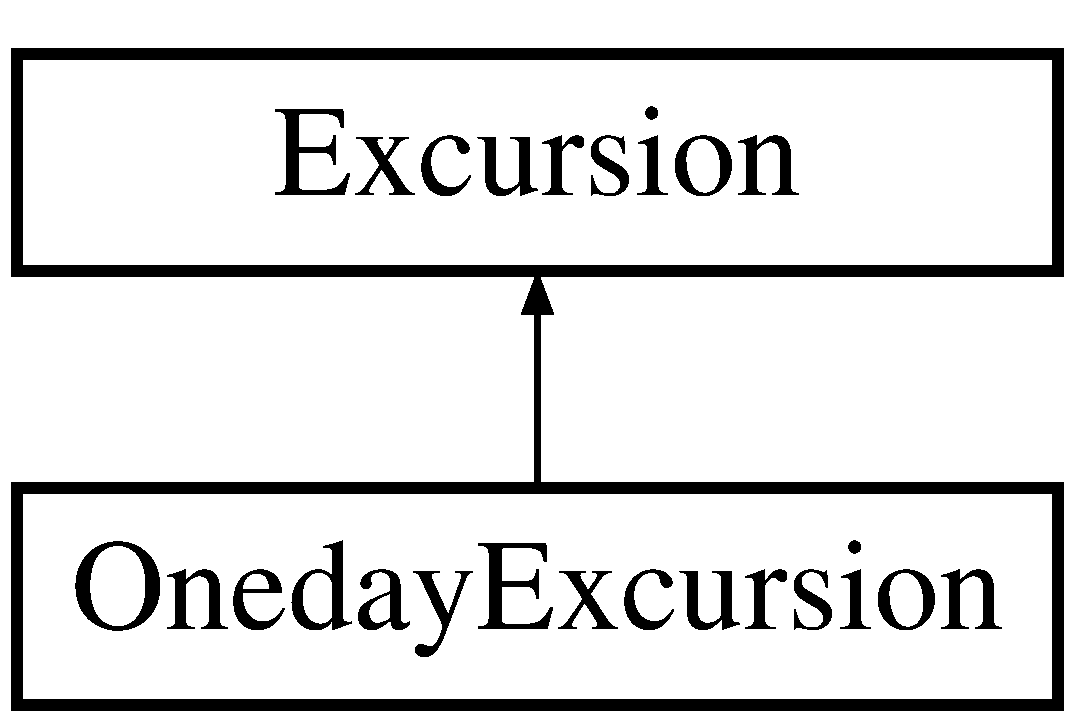
\includegraphics[height=2.000000cm]{class_oneday_excursion}
\end{center}
\end{figure}
\subsection*{Public Member Functions}
\begin{DoxyCompactItemize}
\item 
\hypertarget{class_oneday_excursion_a1ac2c8f44be8ad9294a0c601d4ec3f21}{}\hyperlink{class_oneday_excursion_a1ac2c8f44be8ad9294a0c601d4ec3f21}{Oneday\+Excursion} (const string \&name, const float \&cost, const unsigned int \&year, const unsigned int \&month, const unsigned int \&day, const unsigned int \&hour, const unsigned int \&min, const unsigned int \&max\+Tourists, const unsigned int \&sold\+Seats)\label{class_oneday_excursion_a1ac2c8f44be8ad9294a0c601d4ec3f21}

\begin{DoxyCompactList}\small\item\em конструктор однодневной экскурсии по умолчанию \end{DoxyCompactList}\item 
\hypertarget{class_oneday_excursion_af0a903573c4e4470fddd3183c2eae30e}{}\hyperlink{class_oneday_excursion_af0a903573c4e4470fddd3183c2eae30e}{Oneday\+Excursion} (const string \&name, const float \&cost, const unsigned int \&year, const unsigned int \&month, const unsigned int \&day, const unsigned int \&hour, const unsigned int \&min, const unsigned int \&max\+Tourists, const unsigned int \&sold\+Seats, const \hyperlink{class_route}{Route} \&route)\label{class_oneday_excursion_af0a903573c4e4470fddd3183c2eae30e}

\begin{DoxyCompactList}\small\item\em конструктор однодневной экскурсии \end{DoxyCompactList}\item 
\hypertarget{class_oneday_excursion_a086bfa348889e493e3a1e32d504f442e}{}\hyperlink{class_oneday_excursion_a086bfa348889e493e3a1e32d504f442e}{$\sim$\+Oneday\+Excursion} ()\label{class_oneday_excursion_a086bfa348889e493e3a1e32d504f442e}

\begin{DoxyCompactList}\small\item\em конструктор однодневной экскурсии \end{DoxyCompactList}\item 
\hypertarget{class_oneday_excursion_ac30696f6a7a717f0252001e8454f7341}{}virtual \hyperlink{class_oneday_excursion}{Oneday\+Excursion} $\ast$ \hyperlink{class_oneday_excursion_ac30696f6a7a717f0252001e8454f7341}{clone} () const \label{class_oneday_excursion_ac30696f6a7a717f0252001e8454f7341}

\begin{DoxyCompactList}\small\item\em деструктор однодневной экскурсии \end{DoxyCompactList}\item 
\hypertarget{class_oneday_excursion_aa9379cb2bcc8d6bd5ec832ec438bfcff}{}void \hyperlink{class_oneday_excursion_aa9379cb2bcc8d6bd5ec832ec438bfcff}{set\+Route} (const \hyperlink{class_route}{Route} \&route)\label{class_oneday_excursion_aa9379cb2bcc8d6bd5ec832ec438bfcff}

\begin{DoxyCompactList}\small\item\em метод клонирующий эксукрсию \end{DoxyCompactList}\item 
\hypertarget{class_oneday_excursion_ac000b64a432e5d629c146c67afebc572}{}\hyperlink{class_route}{Route} \& \hyperlink{class_oneday_excursion_ac000b64a432e5d629c146c67afebc572}{get\+Route} ()\label{class_oneday_excursion_ac000b64a432e5d629c146c67afebc572}

\begin{DoxyCompactList}\small\item\em ввод маршрута \end{DoxyCompactList}\end{DoxyCompactItemize}
\subsection*{Protected Member Functions}
\begin{DoxyCompactItemize}
\item 
\hypertarget{class_oneday_excursion_a50e0efe6531857972e72d8085a36e3c5}{}virtual std\+::ostream \& \hyperlink{class_oneday_excursion_a50e0efe6531857972e72d8085a36e3c5}{show} (std\+::ostream \&os) const \label{class_oneday_excursion_a50e0efe6531857972e72d8085a36e3c5}

\begin{DoxyCompactList}\small\item\em перегруженный оператор ввода \end{DoxyCompactList}\item 
\hypertarget{class_oneday_excursion_a7138aa029f429ccde71a79706bcf9f89}{}virtual std\+::istream \& \hyperlink{class_oneday_excursion_a7138aa029f429ccde71a79706bcf9f89}{get} (std\+::istream \&is)\label{class_oneday_excursion_a7138aa029f429ccde71a79706bcf9f89}

\begin{DoxyCompactList}\small\item\em вывод информации об однодневной экскурсии \end{DoxyCompactList}\end{DoxyCompactItemize}
\subsection*{Friends}
\begin{DoxyCompactItemize}
\item 
\hypertarget{class_oneday_excursion_a7e5f8b5bcaa5cdc59c3629e0b7e0f385}{}std\+::ostream \& \hyperlink{class_oneday_excursion_a7e5f8b5bcaa5cdc59c3629e0b7e0f385}{operator$<$$<$} (std\+::ostream \&os, const \hyperlink{class_oneday_excursion}{Oneday\+Excursion} \&oneday\+Excursion)\label{class_oneday_excursion_a7e5f8b5bcaa5cdc59c3629e0b7e0f385}

\begin{DoxyCompactList}\small\item\em вывод маршрута \end{DoxyCompactList}\item 
\hypertarget{class_oneday_excursion_af62b98b24ab8a6fc6401bf6c015c3cdc}{}std\+::istream \& \hyperlink{class_oneday_excursion_af62b98b24ab8a6fc6401bf6c015c3cdc}{operator$>$$>$} (std\+::istream \&is, \hyperlink{class_oneday_excursion}{Oneday\+Excursion} \&oneday\+Excursion)\label{class_oneday_excursion_af62b98b24ab8a6fc6401bf6c015c3cdc}

\begin{DoxyCompactList}\small\item\em перегруженный оператор вывода \end{DoxyCompactList}\end{DoxyCompactItemize}


The documentation for this class was generated from the following files\+:\begin{DoxyCompactItemize}
\item 
oneday\+\_\+excursion.\+h\item 
oneday\+\_\+excursion.\+cpp\end{DoxyCompactItemize}

\hypertarget{struct_record}{}\section{Record Struct Reference}
\label{struct_record}\index{Record@{Record}}
\subsection*{Public Member Functions}
\begin{DoxyCompactItemize}
\item 
\hypertarget{struct_record_a55324487fe8ddb6d260feba8864cc7eb}{}\hyperlink{struct_record_a55324487fe8ddb6d260feba8864cc7eb}{Record} (const \hyperlink{struct_record}{Record} \&record)\label{struct_record_a55324487fe8ddb6d260feba8864cc7eb}

\begin{DoxyCompactList}\small\item\em конструктор структуры, состоящей из кода экскурсии и указателя на экскурсию \end{DoxyCompactList}\end{DoxyCompactItemize}
\subsection*{Public Attributes}
\begin{DoxyCompactItemize}
\item 
\hypertarget{struct_record_ae50469fdf54274743b79f79346b1379a}{}unsigned int {\bfseries code}\label{struct_record_ae50469fdf54274743b79f79346b1379a}

\item 
\hypertarget{struct_record_a614dffcf1864b1dee1902ff78dce681b}{}\hyperlink{class_excursion}{Excursion} $\ast$ {\bfseries excursion}\label{struct_record_a614dffcf1864b1dee1902ff78dce681b}

\end{DoxyCompactItemize}


The documentation for this struct was generated from the following files\+:\begin{DoxyCompactItemize}
\item 
record.\+h\item 
record.\+cpp\end{DoxyCompactItemize}

\hypertarget{class_route}{}\section{Route Class Reference}
\label{class_route}\index{Route@{Route}}
\subsection*{Public Member Functions}
\begin{DoxyCompactItemize}
\item 
\hypertarget{class_route_ad5f4fe1d852768a60246dae8a4862699}{}\hyperlink{class_route_ad5f4fe1d852768a60246dae8a4862699}{Route} (const unsigned int \&amount\+Items)\label{class_route_ad5f4fe1d852768a60246dae8a4862699}

\begin{DoxyCompactList}\small\item\em конструктор маршрута по умолчанию \end{DoxyCompactList}\item 
\hypertarget{class_route_a0f5d78e43214bafb3d973bae07381f58}{}\hyperlink{class_route_a0f5d78e43214bafb3d973bae07381f58}{Route} (const \hyperlink{class_item}{Item} \&item)\label{class_route_a0f5d78e43214bafb3d973bae07381f58}

\begin{DoxyCompactList}\small\item\em контруктор маршрута по количеству экскурсиооных объектов \end{DoxyCompactList}\item 
\hypertarget{class_route_a4d2d48d0fc726775b1f5309a56a8ceef}{}\hyperlink{class_route_a4d2d48d0fc726775b1f5309a56a8ceef}{Route} (const unsigned int \&amount\+Items, \hyperlink{class_item}{Item} $\ast$items)\label{class_route_a4d2d48d0fc726775b1f5309a56a8ceef}

\begin{DoxyCompactList}\small\item\em конструктор маршрута по экскурсиооному объекту \end{DoxyCompactList}\item 
\hypertarget{class_route_a12e053892cff175232b9df34b8bb9d0c}{}\hyperlink{class_route_a12e053892cff175232b9df34b8bb9d0c}{Route} (const \hyperlink{class_route}{Route} \&route)\label{class_route_a12e053892cff175232b9df34b8bb9d0c}

\begin{DoxyCompactList}\small\item\em конструктор маршрута по экскурсионному объекту и их количеству \end{DoxyCompactList}\item 
\hypertarget{class_route_a41212532f2bce3298d8f9468f82c62ab}{}\hyperlink{class_route_a41212532f2bce3298d8f9468f82c62ab}{$\sim$\+Route} ()\label{class_route_a41212532f2bce3298d8f9468f82c62ab}

\begin{DoxyCompactList}\small\item\em копирующий конструктор маршрута \end{DoxyCompactList}\item 
\hypertarget{class_route_ada2034f9fafbe545ee52cd508c2857c3}{}void \hyperlink{class_route_ada2034f9fafbe545ee52cd508c2857c3}{set\+Amount\+Items} (const unsigned int \&amount\+Items)\label{class_route_ada2034f9fafbe545ee52cd508c2857c3}

\begin{DoxyCompactList}\small\item\em деструктор маршрута \end{DoxyCompactList}\item 
\hypertarget{class_route_af4c2579eea10597f0f13d4fd3857b97f}{}void \hyperlink{class_route_af4c2579eea10597f0f13d4fd3857b97f}{set\+Amount\+Items} (std\+::istream \&is)\label{class_route_af4c2579eea10597f0f13d4fd3857b97f}

\begin{DoxyCompactList}\small\item\em ввод количества экскурсионных объектов \end{DoxyCompactList}\item 
\hypertarget{class_route_a9902364fc0bc42d74903895d6f69aacf}{}void \hyperlink{class_route_a9902364fc0bc42d74903895d6f69aacf}{set\+Item} (const unsigned int \&n, const \hyperlink{class_item}{Item} \&item)\label{class_route_a9902364fc0bc42d74903895d6f69aacf}

\begin{DoxyCompactList}\small\item\em ввод количества экскурсионных объектов в поток \end{DoxyCompactList}\item 
\hypertarget{class_route_af01e53eee5dee6ef8285ac651d39b379}{}\hyperlink{class_item}{Item} \& \hyperlink{class_route_af01e53eee5dee6ef8285ac651d39b379}{get\+Item} (const unsigned int \&n)\label{class_route_af01e53eee5dee6ef8285ac651d39b379}

\begin{DoxyCompactList}\small\item\em ввод данных экскурсионного объекта \end{DoxyCompactList}\item 
\hypertarget{class_route_a99bd00c3c6e2f1307a0375e85649c181}{}tm \hyperlink{class_route_a99bd00c3c6e2f1307a0375e85649c181}{get\+Time\+Start} () const \label{class_route_a99bd00c3c6e2f1307a0375e85649c181}

\begin{DoxyCompactList}\small\item\em вывод данных экскурсиооного объекта \end{DoxyCompactList}\item 
\hypertarget{class_route_ab9bea74aecfe030ca9a0f50bb49c3e51}{}unsigned int \hyperlink{class_route_ab9bea74aecfe030ca9a0f50bb49c3e51}{get\+Amount\+Items} () const \label{class_route_ab9bea74aecfe030ca9a0f50bb49c3e51}

\begin{DoxyCompactList}\small\item\em вывод времени начала экскурсиооного объекта \end{DoxyCompactList}\item 
\hypertarget{class_route_a11f4c59d213f85f0608f6ef33cef50c4}{}unsigned int \hyperlink{class_route_a11f4c59d213f85f0608f6ef33cef50c4}{get\+Duration} () const \label{class_route_a11f4c59d213f85f0608f6ef33cef50c4}

\begin{DoxyCompactList}\small\item\em вывод количества экскурсиооных объектов \end{DoxyCompactList}\item 
\hypertarget{class_route_a2687322060916cafbd3f5c848a0512ba}{}\hyperlink{class_route}{Route} \& \hyperlink{class_route_a2687322060916cafbd3f5c848a0512ba}{operator=} (const \hyperlink{class_route}{Route} \&route)\label{class_route_a2687322060916cafbd3f5c848a0512ba}

\begin{DoxyCompactList}\small\item\em вывод продолжительности экскурсии \end{DoxyCompactList}\end{DoxyCompactItemize}
\subsection*{Friends}
\begin{DoxyCompactItemize}
\item 
\hypertarget{class_route_a94d3389e7e325aa8f7394d34db5a33e0}{}std\+::ostream \& \hyperlink{class_route_a94d3389e7e325aa8f7394d34db5a33e0}{operator$<$$<$} (std\+::ostream \&os, const \hyperlink{class_route}{Route} \&route)\label{class_route_a94d3389e7e325aa8f7394d34db5a33e0}

\begin{DoxyCompactList}\small\item\em перегруженный оператор присваивания \end{DoxyCompactList}\item 
\hypertarget{class_route_a48a68fb58c2b4902ca84058f33303c36}{}std\+::istream \& \hyperlink{class_route_a48a68fb58c2b4902ca84058f33303c36}{operator$>$$>$} (std\+::istream \&is, \hyperlink{class_route}{Route} \&route)\label{class_route_a48a68fb58c2b4902ca84058f33303c36}

\begin{DoxyCompactList}\small\item\em перегруженный оператор вывода \end{DoxyCompactList}\end{DoxyCompactItemize}


The documentation for this class was generated from the following file\+:\begin{DoxyCompactItemize}
\item 
route.\+h\end{DoxyCompactItemize}

\hypertarget{class_table_iterator}{}\section{Table\+Iterator Class Reference}
\label{class_table_iterator}\index{Table\+Iterator@{Table\+Iterator}}
\subsection*{Public Member Functions}
\begin{DoxyCompactItemize}
\item 
\hypertarget{class_table_iterator_a0f308b7f879debb2c904b6bfac10a663}{}{\bfseries Table\+Iterator} (\hyperlink{struct_record}{Record} $\ast$current\+Record)\label{class_table_iterator_a0f308b7f879debb2c904b6bfac10a663}

\item 
\hypertarget{class_table_iterator_a4936bda5654819e458172819485bd6ab}{}\hyperlink{struct_record}{Record} \& {\bfseries operator$\ast$} ()\label{class_table_iterator_a4936bda5654819e458172819485bd6ab}

\item 
\hypertarget{class_table_iterator_ac35c71a476d3963253c3cedea51bcbbf}{}\hyperlink{class_table_iterator}{Table\+Iterator} \& {\bfseries operator++} ()\label{class_table_iterator_ac35c71a476d3963253c3cedea51bcbbf}

\item 
\hypertarget{class_table_iterator_a06880f5bc0dce10bc5204019f761f739}{}\hyperlink{class_table_iterator}{Table\+Iterator} {\bfseries operator++} (int)\label{class_table_iterator_a06880f5bc0dce10bc5204019f761f739}

\item 
\hypertarget{class_table_iterator_af52fe40df7ab5c15276bbefb7780352b}{}int {\bfseries operator!=} (const \hyperlink{class_table_iterator}{Table\+Iterator} \&table\+Itarator) const \label{class_table_iterator_af52fe40df7ab5c15276bbefb7780352b}

\item 
\hypertarget{class_table_iterator_a9cbd732fdf6da4594148e8d8746c83fc}{}int {\bfseries operator==} (const \hyperlink{class_table_iterator}{Table\+Iterator} \&table\+Tterator) const \label{class_table_iterator_a9cbd732fdf6da4594148e8d8746c83fc}

\end{DoxyCompactItemize}


The documentation for this class was generated from the following file\+:\begin{DoxyCompactItemize}
\item 
table\+\_\+iterator.\+h\end{DoxyCompactItemize}

\hypertarget{class_vector_table}{}\section{Vector\+Table Class Reference}
\label{class_vector_table}\index{Vector\+Table@{Vector\+Table}}
\subsection*{Public Member Functions}
\begin{DoxyCompactItemize}
\item 
\hypertarget{class_vector_table_a4fcace919113d3adfb809695ea13316d}{}void {\bfseries add\+Record} (const unsigned int \&code, \hyperlink{class_excursion}{Excursion} \&excursion)\label{class_vector_table_a4fcace919113d3adfb809695ea13316d}

\item 
\hypertarget{class_vector_table_a9e4807907bde24f1117cc145c205ce6f}{}void {\bfseries add\+Record} (const unsigned int \&code, const unsigned int \&year, const unsigned int \&month, const unsigned int \&day)\label{class_vector_table_a9e4807907bde24f1117cc145c205ce6f}

\item 
\hypertarget{class_vector_table_a51660a0ee1126898067435ef3f17f52c}{}void {\bfseries add\+Record} (\hyperlink{struct_record}{Record} \&record)\label{class_vector_table_a51660a0ee1126898067435ef3f17f52c}

\item 
\hypertarget{class_vector_table_a98a31837b266e9b6b1f579e5e13b2dbc}{}std\+::vector$<$ \hyperlink{struct_record}{Record} $>$\+::iterator {\bfseries find} (const unsigned int \&code, const unsigned int \&year, const unsigned int \&month, const unsigned int \&day)\label{class_vector_table_a98a31837b266e9b6b1f579e5e13b2dbc}

\item 
\hypertarget{class_vector_table_ab0917cb01c58ed061168946beb8e61aa}{}tm {\bfseries Get\+Data} (const unsigned int \&code, const unsigned int \&year, const unsigned int \&month, const unsigned int \&day)\label{class_vector_table_ab0917cb01c58ed061168946beb8e61aa}

\item 
\hypertarget{class_vector_table_a5f144bd1ef44deaa83f981c14434fbe8}{}std\+::string {\bfseries Get\+Name\+Place} (const unsigned int \&code, const unsigned int \&year, const unsigned int \&month, const unsigned int \&day)\label{class_vector_table_a5f144bd1ef44deaa83f981c14434fbe8}

\item 
\hypertarget{class_vector_table_ac7d26230e13f94f50c6f064012e4fadc}{}bool {\bfseries erase} (const unsigned int \&code, const unsigned int \&year, const unsigned int \&month, const unsigned int \&day)\label{class_vector_table_ac7d26230e13f94f50c6f064012e4fadc}

\item 
\hypertarget{class_vector_table_a434d4a994da0298c0de17763b4ba31a4}{}int {\bfseries Sold\+Seats} (const unsigned int \&code, const unsigned int \&year, const unsigned int \&month, const unsigned int \&day)\label{class_vector_table_a434d4a994da0298c0de17763b4ba31a4}

\item 
\hypertarget{class_vector_table_a81b28afda7a5c323a1dbdffd17b4d866}{}void {\bfseries Set\+Data} (std\+::vector$<$ \hyperlink{struct_record}{Record} $>$\+::iterator \&i, const unsigned int \&year, const unsigned int \&month, const unsigned int \&day, const unsigned int \&hour, const unsigned int \&min)\label{class_vector_table_a81b28afda7a5c323a1dbdffd17b4d866}

\item 
\hypertarget{class_vector_table_a4c9eecaa002bc1ebe62fd61c1ef3567f}{}void {\bfseries Get\+All\+Date} (const unsigned int \&code)\label{class_vector_table_a4c9eecaa002bc1ebe62fd61c1ef3567f}

\item 
\hypertarget{class_vector_table_a12f53f971c363ddf5ca9c75c1c8ef0e1}{}std\+::vector$<$ \hyperlink{struct_record}{Record} $>$\+::iterator {\bfseries find\+Closest} (const unsigned int \&code, const unsigned int \&year, const unsigned int \&month, const unsigned int \&day)\label{class_vector_table_a12f53f971c363ddf5ca9c75c1c8ef0e1}

\item 
\hypertarget{class_vector_table_af0f4cf878c18e1d09d5154473f53b61c}{}void {\bfseries Replace} (const unsigned int \&code, const unsigned int \&year, const unsigned int \&month, const unsigned int \&day)\label{class_vector_table_af0f4cf878c18e1d09d5154473f53b61c}

\item 
\hypertarget{class_vector_table_a30c5fe29b1bd9b73d0dff4e41c54afa6}{}void {\bfseries All\+Find} (const unsigned int \&code)\label{class_vector_table_a30c5fe29b1bd9b73d0dff4e41c54afa6}

\end{DoxyCompactItemize}
\subsection*{Friends}
\begin{DoxyCompactItemize}
\item 
\hypertarget{class_vector_table_afcb2d62bcf5439f203a73d334e5492d1}{}std\+::ostream \& {\bfseries operator$<$$<$} (std\+::ostream \&os, const \hyperlink{class_vector_table}{Vector\+Table} \&vector\+Table)\label{class_vector_table_afcb2d62bcf5439f203a73d334e5492d1}

\end{DoxyCompactItemize}


The documentation for this class was generated from the following files\+:\begin{DoxyCompactItemize}
\item 
vector\+\_\+table.\+h\item 
vector\+\_\+table.\+cpp\end{DoxyCompactItemize}

%--- End generated contents ---

% Index
\backmatter
\newpage
\phantomsection
\clearemptydoublepage
\addcontentsline{toc}{chapter}{Index}
\printindex

\end{document}
